\title{CS 472 HW 2}
\author{
        Aaron Havens \\
}
\date{\today}

\documentclass[12pt]{article}
\usepackage{amssymb} %maths
\usepackage{amsmath} %maths
\usepackage{graphicx}
\graphicspath{{figs/}}
\usepackage{qtree}
\begin{document}
\maketitle

\section{Problem 3.6, Russel}
Give a complete problem formulation for each of the following. Choose a formulation
that is precise enough to be implemented. 

\paragraph{\textbf{d.)}} You have three jugs, measuring 12 gallons, 8 gallons, and 3 gallons, and a water faucet. You can fill the jugs up or empty them out from one to another or onto the ground. You
need to measure out exactly one gallon.
\begin{center}
    \begin{tabular}{ | l | p{10cm} |}
    \hline
	Initial State & A 3-dimensional vector $\textbf{jugs} = [a,b,c] $, where at $t_0$ $\text{jugs}= [0,0,0]$\\
	\hline
	Goal State / Test & If either jug \textit{a, b or c} is equal to exactly 1.\\
	\hline
	Successor Function & The vector state can transition by filling or emptying jugs. Ex. $[0,0,0] \rightarrow [12,0,0] 
	\rightarrow [0,0,0]$. The vector can also be modified by emptying jugs into other jugs of different capacity. Ex. $[0,8,0]
	\rightarrow [8,0,0]$ However, if jug \textit{b} at full capacity 8 is added to jug \textit{a} with capacity 12, jug
	\textit{a} simply \textit{overflows}. $[8,8,0]
	\rightarrow [12,0,0]$\\   
	\hline
	Cost Function &\begin{gather*}J = N_{pours} + M_{empties} \\ 
	\text{or perhaps}\\ 
	J = f(N_{pours} + M_{empties}) + g(\text{Gal. Dumped on Floor})
	\end{gather*}.
	\\
	\hline
    \end{tabular}
\end{center}

\section{Problem 3.9, Russel}
The missionaries and cannibals problem is usually stated as follows. Three missionaries
and three cannibals are on one side of a river, along with a boat that can hold one or
two people. Find a way to get everyone to the other side without ever leaving a group of missionaries
in one place outnumbered by the cannibals in that place. This problem is famous in
AI because it was the subject of the first paper that approached problem formulation from an
analytical viewpoint (Amarel, 1968).
\paragraph{a. Formulate the problem precisely, making only those distinctions necessary to ensure a
valid solution. Draw a diagram of the complete state space.}
\begin{center}
    \begin{tabular}{| l | p{10cm} |}
    \hline
	Initial State & A 6-dimensional vector representing the state of missionaries, cannibals and boats on each side 1 and 2 
	$\textbf{S} = [m_1, c_1, b_1, m_2, c2, b_2]$\\
	\hline
	Goal State / Test & If all of people (cannibals and humans) are on side 2. or if $m_2 \wedge c_2 = 3$\\
	\hline
	Successor Function & If $b_i = 1$, you can move at most 2 people ($(m_i + c_i) \leq 2$) total from the ith side to the jth side.
	$[3,3,1,0,0,0] \rightarrow [2,2,0,1,1,1]$. 
	Notice that the ith boat value becomes zero and the jth boat is 1 ($\neg b_i , \neg b_j$). Every successor state 
	must obey the constraint that for any ith side, $m_i \geq c_i$ or that the cannibals can not outnumber missionaries at any time. Also, of course $m_i,\,c_i \geq 0$.\\
	\hline
	Cost function & Number of actions.\\
	\hline
    \end{tabular}
\end{center}
\paragraph{b. Implement and solve the problem optimally using an appropriate search algorithm. Is it
a good idea to check for repeated states?} It may be a good a idea to check for repeated states especially if using a depth-first search method (infinite loop) being that we can assume that given a current state is independent of all previous states. However, this would require a small amount of memory. We could avoid using history by using a breadth-first search strategy, but it turns out that since the state space is so small, the only history ever required to avoid a repeated state is the previous state (2 previous states of successor.
The following implementation uses a depth-first search, checking if a successor state satisfies the following conditions for every node expansion:
\begin{align}
\begin{split}
S_{k+1} \neq S_{k-1} \\
\text{at }k+1: \\
m_1 \geq c_1 \text{ and } m_2 \geq c_2 \\
m_1,\,c_1,\,m_2,\,c_2 \geq 0
\end{split}
\end{align}
It can be observed that the branching factor and state space of allowable states is actually very small. So small infact that they can be exhausted on this page.
\begin{figure}[h]
\begin{center}
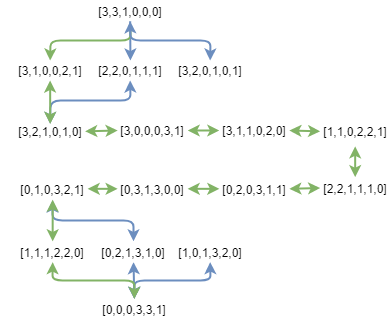
\includegraphics[scale=.75]{c_b_flow}
\caption{The state-space in respect to the cannibal-missionary constraint is relatively small. Shown is \underline{one of the} possible solutions in green (strictly forward from either direction following a depth first search strategy). Either breadth-first or depth-first search will give an optimal solution assuming that your search obeys that the successor state is not the same as the previous state of your current state.}
\end{center}
\end{figure}
\paragraph{c. Why do you think people have a hard time solving this puzzle, given that the state space
is so simple?}
As mentioned before, the branching factor of this 6-D state space may seem large, but after the constraints eq 1 are applied, the number of legal transition states is very small. The legal state space actually collapses into a single path and only branches once more before solution. There are 4 optimal solutions (in respect to number of actions). 
\end{document}